% === A03 - Pila y Convencion C ===
% David Alejandro Gonzalez Marquez
% dmarquez@dc.uba.ar / fokerman@gmail.com
% https://github.com/fokerman/Orga2Course

\documentclass[aspectratio=169]{beamer}
% \documentclass[handout]{beamer}

% % % Packages
\usepackage[sfdefault]{AlegreyaSans}
\usepackage{inconsolata}
\usepackage{multicol}
\usepackage{multirow}
\usepackage[spanish]{babel}
\usepackage[utf8]{inputenc}
\usepackage{enumerate}
\usepackage{color}
\usepackage{xcolor}
\usepackage[absolute,overlay]{textpos}
%   \setlength{\TPHorizModule}{1mm}
%   \setlength{\TPVertModule}{1mm}
\usepackage{framed}
\usepackage{mfirstuc} % para poner en mayusculas la primer letra
\usepackage{xspace} % para crear espacios en comandos 
\usepackage{pbox}
\usepackage{tikz}
\usepackage{mathabx}

% % % Beamer config
\usetheme{Pittsburgh}
\usecolortheme[rgb={1,0.48,0.0}]{structure}
\setbeamercolor{block title}{fg=white,bg=verdeuca}
\xdefinecolor{verdeuca}{rgb}{0.0,0.48,0.54}
\xdefinecolor{naranjauca}{rgb}{1,0.48,0.0}
\setbeamercolor{palette quaternary}{fg=white,bg=verdeuca}
\setbeamertemplate{title page}[default][colsep=-4bp, rounded=true] % remove title shadow
\setbeamertemplate{frametitle}[default][colsep=-2bp, shadow=false] % remove frame title shadow
\setbeamertemplate{navigation symbols}{} % remove navigation symbols
\beamertemplatenavigationsymbolsempty

% % % Colors
\definecolor{AzulClaro}{rgb}{.31,.506,.741}
\definecolor{Gris}{gray}{0.8}
\definecolor{Celeste}{rgb}{.255,.41,.884}
\definecolor{Rojo}{rgb}{1, 0, 0}

% % % Rename
\newcommand{\tab}[0]{\hspace{15pt}}

% % % Blocks
\setbeamercolor{block body}{fg=black, bg=black!10}
\setbeamercolor{block title}{fg=black, bg=black!20}
\setbeamercolor{coloredboxstuffNaranja}{fg=naranjauca,bg=black!10} %% PARA LOS BOX
\setbeamercolor{coloredboxstuffVerde}{fg=verdeuca,bg=black!10} %% PARA LOS BOX

% % % Start

\title{\Huge Pila y Convención C}
\author{David Alejandro González Márquez}
\institute{Departamento de Computación\\
Facultad de Ciencias Exactas y Naturales\\
Universidad de Buenos Aires}
\date{}

\begin{document}

\begin{frame}[plain]
    \titlepage 
\end{frame}

\begin{frame}[fragile]
    \frametitle{Temario}
    \large
    \begin{itemize}
    \setlength\itemsep{0.5cm}
    \item Estructura y uso de la Pila
    \pause
    \item Convención C
    \begin{itemize}
    \item \large Stack Frame y conservación de registros
    \item \large Pasaje de parámetros
    \end{itemize}
    \pause
    \item Ensamblar, compilar y linkear, código C y ASM
    \end{itemize}
\end{frame}

\begin{frame}
    \frametitle{Introducción}
    \begin{itemize}
    \setlength\itemsep{0.5cm}
    \item[-] La pila es una estructura en memoria.
    \pause
    \item[-] Se utiliza para guardar \textbf{información local} a una función.
    \pause
    \item[-] Además sirve para almacenar información de \textbf{contexto}.
    \pause
    \item[-] Tanto en x86 como en x86-64, la pila tiene distintos parámetros.
    \end{itemize}
\end{frame}

\begin{frame}
    \frametitle{Pila - Estructura}
    \begin{textblock}{5}(-4,1.5)
    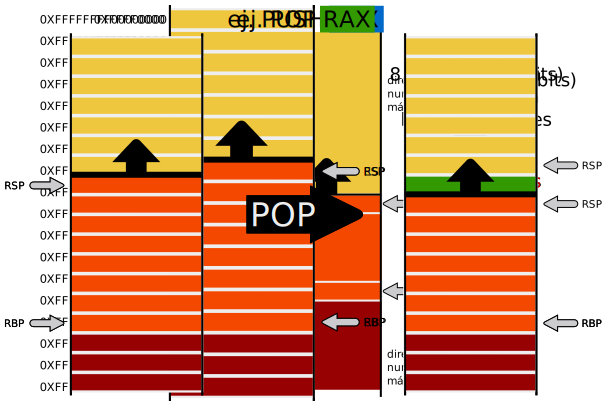
\includegraphics[scale=0.75]{img/pila.pdf}
    \end{textblock}
    \begin{textblock}{9}(7,3)
    \uncover<2->{
    \textcolor{verdeuca}{En 32 bits}
    \begin{itemize}
    \item[-] Los registros \texttt{EBP} y \texttt{ESP}
    \item[-] \textcolor{naranjauca}{\texttt{EBP} (Base Pointer)} apunta a la base
    \item[-] \textcolor{naranjauca}{\texttt{ESP} (Stack Pointer)} al tope (último elemento válido)
    \end{itemize}
    }
    \vspace{1cm}
    \uncover<3->{
    \textcolor{verdeuca}{En 64 bits}
    \begin{itemize}
    \item[-] Los registros \texttt{RBP} y \texttt{RSP}
    \item[-] \textcolor{naranjauca}{\texttt{RBP} (Base Pointer)} apunta a la base
    \item[-] \textcolor{naranjauca}{\texttt{RSP} (Stack Pointer)} al tope (último elemento válido)
    \end{itemize}
    }
    \end{textblock}
\end{frame}

\begin{frame}
    \frametitle{Pila en 32 bits - Estructura}
    \begin{textblock}{5}(1,1.8)
    \includegraphics[scale=0.75]{img/pila-layer2.pdf}
    \end{textblock}
\end{frame}

\begin{frame}
    \frametitle{Pila en 64 bits - Estructura}
    \begin{textblock}{5}(1,1.8)
    \includegraphics[scale=0.75]{img/pila-layer3.pdf}
    \end{textblock}
\end{frame}

\begin{frame}
    \frametitle{Instrucciones}
    \begin{center}
    \vspace{-0.7cm}
    \begin{minipage}{1\textwidth}
    \begin{figure}
    \centering
    \includegraphics[scale=0.73]{img/pila-layer4.pdf}
    \end{figure}
    \end{minipage}
    Operaciones \texttt{PUSH} (apilar) y \texttt{POP} (desapilar)
    \end{center}
\end{frame}

\begin{frame}
    \frametitle{Instrucciones}
    \begin{center}
    \vspace{-0.7cm}
    \begin{minipage}{1\textwidth}
    \begin{figure}
    \centering
    \includegraphics[scale=0.73]{img/pila-layer5.pdf}
    \end{figure}
    \end{minipage}
    Operaciones \texttt{PUSH} (apilar) y \texttt{POP} (desapilar)
    \end{center}
\end{frame}

\begin{frame}{Convención \texttt{C}}
    \begin{itemize}
    \item[-] La forma en que se \textbf{codifican} los llamados a subrutinas en \texttt{C} es estática y depende de la \textbf{firma} de la función a llamar.
    \vspace{0.5cm}
    \pause
    \item[-] De esta forma las funciones pueden ser llamadas sin tener en cuenta como fueron implementadas.
    \vspace{0.5cm}
    \pause
    \item[-] La convención define:
    \begin{itemize}
    \item[$\cdot$] Cómo las funciones \textbf{reciben parámetros}.
    \pause
    \item[$\cdot$] Cómo las funciones \textbf{retornan el resultado}.
    \pause
    \item[$\cdot$] Qué registros se \textbf{deben preservar} en una función.
    \end{itemize}
    \vspace{0.5cm}
    \pause
    \item[-] Las convenciones dependen de la arquitectura del procesador y del sistema operativo:
    \begin{itemize}
    \item[$\cdot$] En \texttt{x86/Linux} (32bits) se conoce como \texttt{x32 ABI}.
    \item[$\cdot$] En \texttt{x86-64/Linux} (64bits) se deomina \texttt{System V AMD64 ABI}.
    \end{itemize}
    \end{itemize}
\end{frame}

\begin{frame}{Stack frame}
    Una función en C es ejecutada dentro de un \textbf{contexto de ejecución}, esté contiene un puntero válido al tope de pila y un puntero a base de pila.
    \vspace{0.5cm}
    \pause
    \begin{block}{stack frame}
    Estructura en memoria constituida por la dirección de retorno, el conjunto de registros preservados, las variables locales y los parámetros pasados por pila.
    \end{block}
    \pause
    \vspace{0.5cm}
    La construcción del \emph{stack frame} consiste en colocar el registro base de la pila en una dirección relativa al comienzo del área de la función llamadora.
\end{frame}

\begin{frame}{Caso 32 bits}
    \begin{itemize}
    \setlength\itemsep{0.3cm}
    \item[-] Preservar los registros \texttt{EBX}, \texttt{ESI}, \texttt{EDI} y \texttt{EBP}\\
    (Se deben preservar SOLO los registros que se modifican).
    \pause
    \item[-] Retornar el resultado a través de \texttt{EAX} (y \texttt{EDX:EAX} si ocupa 64 bits).
    \pause
    \item[-] Preservar la consistencia de la pila.
    \pause
    \item[-] Los parámetros se pasan por pila.
    \pause
    \item[-] La pila debe estar alineada a 4 bytes antes de un llamado a función.
    \end{itemize}
\end{frame}

\begin{frame}{Caso 32 bits}
    \begin{textblock}{20}(3.8,1.0) \only<1->{\includegraphics[scale=0.5]{img/stackframe32-layer1.pdf}} \end{textblock}
    \begin{textblock}{20}(3.8,1.0) \only<3->{\includegraphics[scale=0.5]{img/stackframe32-layer6.pdf}} \end{textblock}
    \begin{textblock}{20}(3.8,1.0) \only<4->{\includegraphics[scale=0.5]{img/stackframe32-layer25.pdf}} \end{textblock}
    \begin{textblock}{20}(3.8,1.0) \only<5->{\includegraphics[scale=0.5]{img/stackframe32-layer26.pdf}} \end{textblock}
    \begin{textblock}{20}(3.8,1.0) \only<6->{\includegraphics[scale=0.5]{img/stackframe32-layer27.pdf}} \end{textblock}
    \begin{textblock}{20}(3.8,1.0) \only<7->{\includegraphics[scale=0.5]{img/stackframe32-layer28.pdf}} \end{textblock}
    \begin{textblock}{20}(3.8,1.0) \only<8->{\includegraphics[scale=0.5]{img/stackframe32-layer29.pdf}} \end{textblock}
    \begin{textblock}{20}(3.8,1.0) \only<9->{\includegraphics[scale=0.5]{img/stackframe32-layer30.pdf}} \end{textblock}
    \begin{textblock}{20}(3.8,1.0) \only<10->{\includegraphics[scale=0.5]{img/stackframe32-layer31.pdf}} \end{textblock}
    \begin{textblock}{20}(3.8,1.0) \only<2-9>{\includegraphics[scale=0.5]{img/stackframe32-layer32.pdf}} \end{textblock}
    \begin{textblock}{20}(3.8,1.0) \only<3-8>{\includegraphics[scale=0.5]{img/stackframe32-layer33.pdf}} \end{textblock}
    \begin{textblock}{20}(3.8,1.0) \only<4-7>{\includegraphics[scale=0.5]{img/stackframe32-layer34.pdf}} \end{textblock}
    \begin{textblock}{20}(3.8,1.0) \only<5-6>{\includegraphics[scale=0.5]{img/stackframe32-layer35.pdf}} \end{textblock}
    \begin{textblock}{20}(3.8,1.0) \only<6-6>{\includegraphics[scale=0.5]{img/stackframe32-layer36.pdf}} \end{textblock}
    \begin{textblock}{20}(3.8,1.0) \only<6-6>{\includegraphics[scale=0.5]{img/stackframe32-layer37.pdf}} \end{textblock}
    \begin{textblock}{20}(3.8,1.0) \only<3-8>{\includegraphics[scale=0.5]{img/stackframe32-layer38.pdf}} \end{textblock}
    \begin{textblock}{20}(3.8,1.0) \only<3-8>{\includegraphics[scale=0.5]{img/stackframe32-layer39.pdf}} \end{textblock}
    \begin{textblock}{20}(3.8,1.0) \only<1->{\includegraphics[scale=0.5]{img/stackframe32-layer40.pdf}} \end{textblock}
\end{frame}

\begin{frame}{Caso 64 bits}
    \begin{itemize}
    \setlength\itemsep{0.3cm}
    \item[-] Preservar los registros \texttt{RBX}, \texttt{R12}, \texttt{R13}, \texttt{R14}, \texttt{R15} y \texttt{RBP}\\
    (Se deben preservar SOLO los registros que se modifican).
    \pause
    \item[-] Retornar el resultado a través de \texttt{RAX} si es un valor entero\\ (y \texttt{RDX:RAX} si ocupa 128bits) o \texttt{XMM0},  si es un número de punto flotante.
    \pause
    \item[-] Preservar la consistencia de la pila.
    \pause
    \item[-] La pila opera alineada a 8 bytes.\\ Pero antes de llamar a funciones de \texttt{C} debe estarlo a \color{red}{\textbf{16 bytes}}\color{black}.
    \end{itemize}
\end{frame}

\begin{frame}{Caso 64 bits}
    \begin{textblock}{20}(3.8,1.0) \only<1->{\includegraphics[scale=0.5]{img/stackframe64-layer1.pdf}} \end{textblock}
    \begin{textblock}{20}(3.8,1.0) \only<3->{\includegraphics[scale=0.5]{img/stackframe64-layer6.pdf}} \end{textblock}
    \begin{textblock}{20}(3.8,1.0) \only<4->{\includegraphics[scale=0.5]{img/stackframe64-layer2.pdf}} \end{textblock}
    \begin{textblock}{20}(3.8,1.0) \only<5->{\includegraphics[scale=0.5]{img/stackframe64-layer3.pdf}} \end{textblock}
    \begin{textblock}{20}(3.8,1.0) \only<6->{\includegraphics[scale=0.5]{img/stackframe64-layer4.pdf}} \end{textblock}
    \begin{textblock}{20}(3.8,1.0) \only<7->{\includegraphics[scale=0.5]{img/stackframe64-layer5.pdf}} \end{textblock}
    \begin{textblock}{20}(3.8,1.0) \only<8->{\includegraphics[scale=0.5]{img/stackframe64-layer7.pdf}} \end{textblock}
    \begin{textblock}{20}(3.8,1.0) \only<9->{\includegraphics[scale=0.5]{img/stackframe64-layer8.pdf}} \end{textblock}
    \begin{textblock}{20}(3.8,1.0) \only<10->{\includegraphics[scale=0.5]{img/stackframe64-layer9.pdf}} \end{textblock}
    \begin{textblock}{20}(3.8,1.0) \only<11->{\includegraphics[scale=0.5]{img/stackframe64-layer10.pdf}} \end{textblock}
    \begin{textblock}{20}(3.8,1.0) \only<2-10>{\includegraphics[scale=0.5]{img/stackframe64-layer11.pdf}} \end{textblock}
    \begin{textblock}{20}(3.8,1.0) \only<3-9>{\includegraphics[scale=0.5]{img/stackframe64-layer12.pdf}} \end{textblock}
    \begin{textblock}{20}(3.8,1.0) \only<5-8>{\includegraphics[scale=0.5]{img/stackframe64-layer13.pdf}} \end{textblock}
    \begin{textblock}{20}(3.8,1.0) \only<6-7>{\includegraphics[scale=0.5]{img/stackframe64-layer14.pdf}} \end{textblock}
    \begin{textblock}{20}(3.8,1.0) \only<4-9>{\includegraphics[scale=0.5]{img/stackframe64-layer15.pdf}} \end{textblock}
    \begin{textblock}{20}(3.8,1.0) \only<7-7>{\includegraphics[scale=0.5]{img/stackframe64-layer16.pdf}} \end{textblock}
    \begin{textblock}{20}(3.8,1.0) \only<4-9>{\includegraphics[scale=0.5]{img/stackframe64-layer17.pdf}} \end{textblock}
    \begin{textblock}{20}(3.8,1.0) \only<1->{\includegraphics[scale=0.5]{img/stackframe64-layer18.pdf}} \end{textblock}
\end{frame}

\begin{frame}{Pasaje de parámetros}
    \textcolor{verdeuca}{En 32 bits}\\
    \begin{itemize}
    \item[-] Los parámetros se pasan \textbf{a través de la pila} desde la dirección más baja a la más alta.
    \pause
    \item[-] Son apilados de derecha a izquierda según aparecen en la firma de la función.
    \pause
    \item[-] Para valores de 64bits se apilan en little-endian.
    \end{itemize}
    \vspace{0.5cm}
    \pause
    \textcolor{verdeuca}{En 64 bits}\\
    \begin{itemize}
    \item[-] Los parámetros \textbf{se pasan por registro}, de izquierda a derecha según la firma de la función, clasificados por tipo:
    \pause
    \begin{itemize}
    \item[$\cdot$] Enteros y direcciónes de memoria: \texttt{RDI}, \texttt{RSI}, \texttt{RDX}, \texttt{RCX}, \texttt{R8} y \texttt{R9}
    \pause
    \item[$\cdot$] Punto flotante: \texttt{XMM0} a \texttt{XMM7}
    \pause
    \item[$\cdot$] Resto de los parámetros que superen la cantidad de registros se ubican en la pila como en 32 bits.
    \end{itemize}
    \end{itemize}
\end{frame}

\begin{frame}[t,fragile]
\frametitle{Ejemplo en 32 bits}
\begin{verbatim}
int f1( int a, float b, double c, int* d, double* e)
\end{verbatim}
    \begin{textblock}{20}(0.5,4) \only<1->{\includegraphics[scale=0.6]{img/ejemplo32-layer1.pdf}} \end{textblock}
    \begin{textblock}{20}(0.5,4) \only<1->{\includegraphics[scale=0.6]{img/ejemplo32-layer7.pdf}} \end{textblock}
    \begin{textblock}{20}(0.5,4) \only<2->{\includegraphics[scale=0.6]{img/ejemplo32-layer8.pdf}} \end{textblock}
    \begin{textblock}{20}(0.5,4) \only<3->{\includegraphics[scale=0.6]{img/ejemplo32-layer9.pdf}} \end{textblock}
    \begin{textblock}{20}(0.5,4) \only<4->{\includegraphics[scale=0.6]{img/ejemplo32-layer10.pdf}} \end{textblock}
    \begin{textblock}{20}(0.5,4) \only<5->{\includegraphics[scale=0.6]{img/ejemplo32-layer11.pdf}} \end{textblock}
    \begin{textblock}{20}(0.5,4) \only<6->{\includegraphics[scale=0.6]{img/ejemplo32-layer12.pdf}} \end{textblock}
    \begin{textblock}{20}(0.5,4) \only<7->{\includegraphics[scale=0.6]{img/ejemplo32-layer13.pdf}} \end{textblock}
    \begin{textblock}{20}(0.5,4) \only<8->{\includegraphics[scale=0.6]{img/ejemplo32-layer15.pdf}} \end{textblock}
    \begin{textblock}{20}(0.5,4) \only<8->{\includegraphics[scale=0.6]{img/ejemplo32-layer2.pdf}} \end{textblock}
    \begin{textblock}{20}(0.5,8.4) \only<1-1>{\includegraphics[scale=0.6]{img/ejemplo32-layer14.pdf}} \end{textblock}
    \begin{textblock}{20}(0.5,7.7) \only<2-2>{\includegraphics[scale=0.6]{img/ejemplo32-layer14.pdf}} \end{textblock}
    \begin{textblock}{20}(0.5,6.9) \only<3-3>{\includegraphics[scale=0.6]{img/ejemplo32-layer14.pdf}} \end{textblock}
    \begin{textblock}{20}(0.5,6.2) \only<4-4>{\includegraphics[scale=0.6]{img/ejemplo32-layer14.pdf}} \end{textblock}
    \begin{textblock}{20}(0.5,5.5) \only<5-5>{\includegraphics[scale=0.6]{img/ejemplo32-layer14.pdf}} \end{textblock}
    \begin{textblock}{20}(0.5,4.7) \only<6-6>{\includegraphics[scale=0.6]{img/ejemplo32-layer14.pdf}} \end{textblock}
    \begin{textblock}{20}(0.5,4)    \only<7->{\includegraphics[scale=0.6]{img/ejemplo32-layer14.pdf}} \end{textblock}
    \begin{textblock}{20}(0.5,4) \only<1->{\includegraphics[scale=0.6]{img/ejemplo32-layer16.pdf}} \end{textblock}
\end{frame}

\begin{frame}[t,fragile]
\frametitle{Ejemplo en 64 bits}
\begin{verbatim}
int f1( int a, float b, double c, int* d, double* e)
\end{verbatim}
    \begin{textblock}{20}(2.0,6) \only<7->{\includegraphics[scale=0.45]{img/ejemplo64-1-layer1.pdf}} \end{textblock}
    \begin{textblock}{20}(2.0,6) \only<1->{\includegraphics[scale=0.45]{img/ejemplo64-1-layer7.pdf}} \end{textblock}
    \begin{textblock}{20}(2.0,6) \only<2->{\includegraphics[scale=0.45]{img/ejemplo64-1-layer8.pdf}} \end{textblock}
    \begin{textblock}{20}(2.0,6) \only<3->{\includegraphics[scale=0.45]{img/ejemplo64-1-layer9.pdf}} \end{textblock}
    \begin{textblock}{20}(2.0,6) \only<4->{\includegraphics[scale=0.45]{img/ejemplo64-1-layer10.pdf}} \end{textblock}
    \begin{textblock}{20}(2.0,6) \only<5->{\includegraphics[scale=0.45]{img/ejemplo64-1-layer11.pdf}} \end{textblock}
    \begin{textblock}{20}(2.0,6) \only<6->{\includegraphics[scale=0.45]{img/ejemplo64-1-layer12.pdf}} \end{textblock}
\end{frame}

\begin{frame}[t,fragile]
\frametitle{Ejemplo en 64 bits}
\begin{verbatim}
int f( int a1, float a2, double a3, int a4, float a5,
double a6, int* a7, double* a8, int* a9, double a10,
int** a11, float* a12, double** a13, int* a14, float a15)
\end{verbatim}
    \begin{textblock}{20}(2.0,6) \only<17->{\includegraphics[scale=0.45]{img/ejemplo64-2-layer1.pdf}} \end{textblock}
    \begin{textblock}{20}(2.0,6) \only<1->{\includegraphics[scale=0.45]{img/ejemplo64-2-layer7.pdf}} \end{textblock}
    \begin{textblock}{20}(2.0,6) \only<2->{\includegraphics[scale=0.45]{img/ejemplo64-2-layer8.pdf}} \end{textblock}
    \begin{textblock}{20}(2.0,6) \only<3->{\includegraphics[scale=0.45]{img/ejemplo64-2-layer9.pdf}} \end{textblock}
    \begin{textblock}{20}(2.0,6) \only<4->{\includegraphics[scale=0.45]{img/ejemplo64-2-layer10.pdf}} \end{textblock}
    \begin{textblock}{20}(2.0,6) \only<5->{\includegraphics[scale=0.45]{img/ejemplo64-2-layer11.pdf}} \end{textblock}
    \begin{textblock}{20}(2.0,6) \only<6->{\includegraphics[scale=0.45]{img/ejemplo64-2-layer12.pdf}} \end{textblock}
    \begin{textblock}{20}(2.0,6) \only<7->{\includegraphics[scale=0.45]{img/ejemplo64-2-layer13.pdf}} \end{textblock}
    \begin{textblock}{20}(2.0,6) \only<8->{\includegraphics[scale=0.45]{img/ejemplo64-2-layer14.pdf}} \end{textblock}
    \begin{textblock}{20}(2.0,6) \only<9->{\includegraphics[scale=0.45]{img/ejemplo64-2-layer15.pdf}} \end{textblock}
    \begin{textblock}{20}(2.0,6) \only<10->{\includegraphics[scale=0.45]{img/ejemplo64-2-layer16.pdf}} \end{textblock}
    \begin{textblock}{20}(2.0,6) \only<11->{\includegraphics[scale=0.45]{img/ejemplo64-2-layer17.pdf}} \end{textblock}
    \begin{textblock}{20}(2.0,6) \only<12->{\includegraphics[scale=0.45]{img/ejemplo64-2-layer18.pdf}} \end{textblock}
    \begin{textblock}{20}(2.0,6) \only<13->{\includegraphics[scale=0.45]{img/ejemplo64-2-layer5.pdf}} \end{textblock}
    % PILA
    \begin{textblock}{20}(2.0,4.75) \only<14-14>{\includegraphics[scale=0.45]{img/ejemplo64-2-layer4.pdf}} \end{textblock}
    \begin{textblock}{20}(2.0,5.4) \only<15-15>{\includegraphics[scale=0.45]{img/ejemplo64-2-layer4.pdf}} \end{textblock}
    \begin{textblock}{20}(2.0,5.4) \only<15-15>{\includegraphics[scale=0.45]{img/ejemplo64-2-layer3.pdf}} \end{textblock}
    \begin{textblock}{20}(2.0,6) \only<16->{\includegraphics[scale=0.45]{img/ejemplo64-2-layer2.pdf}} \end{textblock}
    \begin{textblock}{20}(2.0,6) \only<16->{\includegraphics[scale=0.45]{img/ejemplo64-2-layer3.pdf}} \end{textblock}
    \begin{textblock}{20}(2.0,6) \only<16->{\includegraphics[scale=0.45]{img/ejemplo64-2-layer4.pdf}} \end{textblock}
    \begin{textblock}{20}(2.0,6) \only<1->{\includegraphics[scale=0.45]{img/ejemplo64-2-layer6.pdf}} \end{textblock}
\end{frame}

\begin{frame}[fragile]
\frametitle{Interacción \texttt{C}-\texttt{ASM} - \textbf{Llamar a funciones \texttt{ASM} desde \texttt{C}}}
\small
\texttt{global} indica que el simbolo \texttt{fun} es visible desde el exterior del \texttt{ASM}.\\
\texttt{extern} permite declarar la firma \texttt{fun} para luego ser linkeada.\\
\normalsize
\medskip
\begin{columns}
\column{2.0in}
\begin{block}{funcion.asm}
\vspace{-0.5cm}
\begin{verbatim}
global fun
section .text
fun:
    ...
    ...
    ret
\end{verbatim}
\vspace{-0.3cm}
\end{block}
\column{2.0in}
\begin{block}{programa.c}
\vspace{-0.5cm}
\begin{verbatim}
extern int fun(int, int);
int main(){
    ...
    fun(44,3);
    ..
}
\end{verbatim}
\vspace{-0.3cm}
\end{block}
\end{columns}
\pause
\medskip
\begin{enumerate}
 \item Ensamblar código \texttt{ASM}:\\
 \texttt{nasm -f elf64 funcion.asm -o funcion.o}
 \item Compilar y linkear el código \texttt{C}:\\
 \texttt{gcc -o ejec programa.c funcion.o}
\end{enumerate}
\end{frame}

\begin{frame}[fragile]
\frametitle{Interacción \texttt{C}-\texttt{ASM} - \textbf{Llamar funciones \texttt{C} desde \texttt{ASM}}}
\texttt{extern} indica que el simbolo no esta definido en el \texttt{ASM}:
% \medskip
\begin{small}
\begin{columns}
\column{2.0in}
\begin{block}{main.asm}
\vspace{-0.5cm}
\begin{verbatim}
global main
extern fun
section .text
main:
    ...
    call fun
    ...
    ret
\end{verbatim}
\vspace{-0.3cm}
\end{block}

\column{2.0in}
\begin{block}{funcion.c}
\vspace{-0.5cm}
\begin{verbatim}
int fun(int a, int b){
    ...
    ...
    int res = a + b;
    ...
    return res;

}
\end{verbatim}
\vspace{-0.3cm}
\end{block}
\end{columns}
\end{small}
\pause
\medskip
\begin{enumerate}
\item Ensamblar código \texttt{ASM}:\\
\texttt{nasm -f elf64 main.asm -o main.o}
\item Compilar código \texttt{C} en un objeto\\
\texttt{gcc -no-pie \textbf{-c} -m64 funcion.c -o funcion.o}
\item Usar \texttt{gcc} como linker de ambos archivos objeto.\\
\texttt{gcc -no-pie -o ejec -m64 main.o funcion.o}
\end{enumerate}
\end{frame}

\begin{frame}
    \frametitle{Notas: Alineación}
    \begin{enumerate}
    \setlength\itemsep{0.5cm}
    \item Antes de llamar a una función la pila debe estar alineada a 16 bytes.
    \pause
    \item Al entrar a una función, se guarda en la pila la dirección de retorno, por lo tanto queda desalineada. Ya que la dirección de retorno ocupa un lugar en la pila, es decir 8 bytes.
    \pause
    \item Al ejecutar \texttt{push} \texttt{rbp} la pila vuelve a quedar alineada a 16 bytes.
    \end{enumerate}
    \pause
    \bigskip
    Recordar alinear la pila a 16 bytes antes de llamar a una función.\\
    \textcolor{verdeuca}{Esto se debe realizar por convención.}
\end{frame}

\begin{frame}[fragile]
    \frametitle{Notas: Funciones variádicas (de aridad variable)}
    \pause
    Para estas funciones toman una \textbf{cantidad variable de parámetros}.
    Depende como estén implementadas, identifican la cantidad de parámetros pasados.\\
    \pause
    \bigskip
    \textbf{Caso}: \texttt{printf}\\
    \bigskip
    \texttt{printf(char* formato, ...)}\\
    \pause
    \bigskip
    \textcolor{verdeuca}{Ejemplo}:
    \bigskip
    \includegraphics[scale=1]{img/printf.pdf}

    % \small Donde \texttt{valor} = 45 y \texttt{nombre} = Licuadora\\
    % \normalsize
    % \verb|printf("Item %s : Numero %i", nombre, valor)|\\
    % \bigskip
    % \textcolor{verdeuca}{Resultado}\\
    % Item Licuadora : Numero 45\\
    % \bigskip
    \pause
    \textcolor{verdeuca}{IMPORTANTE: Desde ASM}\\
    Se debe pasar en \texttt{RAX} el número 1, si se va a imprimir valores en punto flotante.\\
    % EN REALIDAD RAX DE CONTENER LA CANTIDAD DE PARAMETROS XMMs PASADOS A PRINTF, PERO EN GRAL CON RAX=1 SOBRA... SI NO REVIENTA!
    % \\ \bigskip
    %  {\tiny [*] http://www.cplusplus.com/reference/clibrary/cstdio/printf/}\\
    \small \textcolor{verdeuca}{Además:} Usar el flag \texttt{-no-pie} para que el linker use símbolos estáticos (ver bibliográfica)
\end{frame}

\begin{frame}[fragile]
    \frametitle{Ejercicios}
    \small
    \begin{enumerate}
    % \item Ensamblar y ejecutar el ejemplo de ``\texttt{Hola Mundo}'' en \texttt{ASM}.
    % \medskip
    \item Armar un programa en \texttt{C} que llame a una función en \texttt{ASM} que sume dos enteros. La de función \texttt{C} debe imprimir el resultado.
    \medskip
    \item Modificar la función anterior para que sume dos numeros de tipo \texttt{double} (ver instrucción \texttt{ADDPD}).
    \medskip
    \item Construir una función en \texttt{ASM} que imprima correctamente por pantalla sus parámetros en orden, llamando sólo una vez a \texttt{printf}. La función debe tener la siguiente aridad: \\
    \verb=void imprime_parametros( int a, double f, char* s );=
    \medskip
    \item Construir una función en \texttt{ASM} con la siguiente aridad: \\
    \footnotesize
    \verb=int suma_parametros( int a0, int a1, int a2, int a3,=
    \verb=                     int a4, int a5 ,int a6, int a7 );=\\
    \small
    Ésta retorna el resultado de la operación: \\
    \footnotesize
    \verb=a0-a1+a2-a3+a4-a5+a6-a7=
    \end{enumerate}
    \normalsize
\end{frame}

\begin{frame}[fragile]
    \frametitle{Bibliografía: Fuentes y material adicional}
    \begin{itemize}
    \item Convenciones de llamados a función en x86: \\
    \url{https://en.wikipedia.org/wiki/X86_calling_conventions}
    \item Notas sobre System V ABI: \\
    \url{https://wiki.osdev.org/System_V_ABI}
    \item Documentación de NASM: \\
    \url{https://nasm.us/doc/}
    \item Artículo sobre el flag \texttt{-pie}: \\
    \url{https://eklitzke.org/position-independent-executables}
    \item Documentación de System V ABI: \\
    \url{https://uclibc.org/docs/psABI-x86_64.pdf}
    \item Manuales de Intel: \\
    \url{https://software.intel.com/en-us/articles/intel-sdm}
    \end{itemize}
\end{frame}

\begin{frame}[plain]
    \begin{center}
    \vspace{2cm}
    \huge ¡Gracias!\\
    \vspace{2cm}
    \normalsize Recuerden leer los comentarios al final de \\ este video por aclaraciones o fe de erratas.
    \end{center}
\end{frame}

\end{document}

